\documentclass{article}%
\usepackage[T1]{fontenc}%
\usepackage[utf8]{inputenc}%
\usepackage{lmodern}%
\usepackage{textcomp}%
\usepackage{lastpage}%
\usepackage[head=40pt,margin=0.5in,bottom=0.6in]{geometry}%
\usepackage{graphicx}%
%
\title{\textbf{El Parlamento regional catalán quiere investigar la monarquía española}}%
\author{AFP}%
\date{07/03/2019}%
%
\begin{document}%
\normalsize%
\maketitle%
\textbf{URL: }%
http://www.eluniversal.com/internacional/34981/el{-}parlamento{-}regional{-}catalan{-}quiere{-}investigar{-}la{-}monarquia{-}espanola\newline%
%
\textbf{Periodico: }%
EU, %
ID: %
34981, %
Seccion: %
internacional\newline%
%
\textbf{Palabras Claves: }%
NO\_TIENE\newline%
%
\textbf{Derecho: }%
2.1%
, Otros Derechos: %
\newline%
%
\textbf{\textit{La propuesta de resolución, aprobada con 71 votos a favor y 56 en contra, acuerda investigar "las actividades irregulares o delictivas de personas vinculadas a la Familia Real"}}%
\newline%
\newline%
%
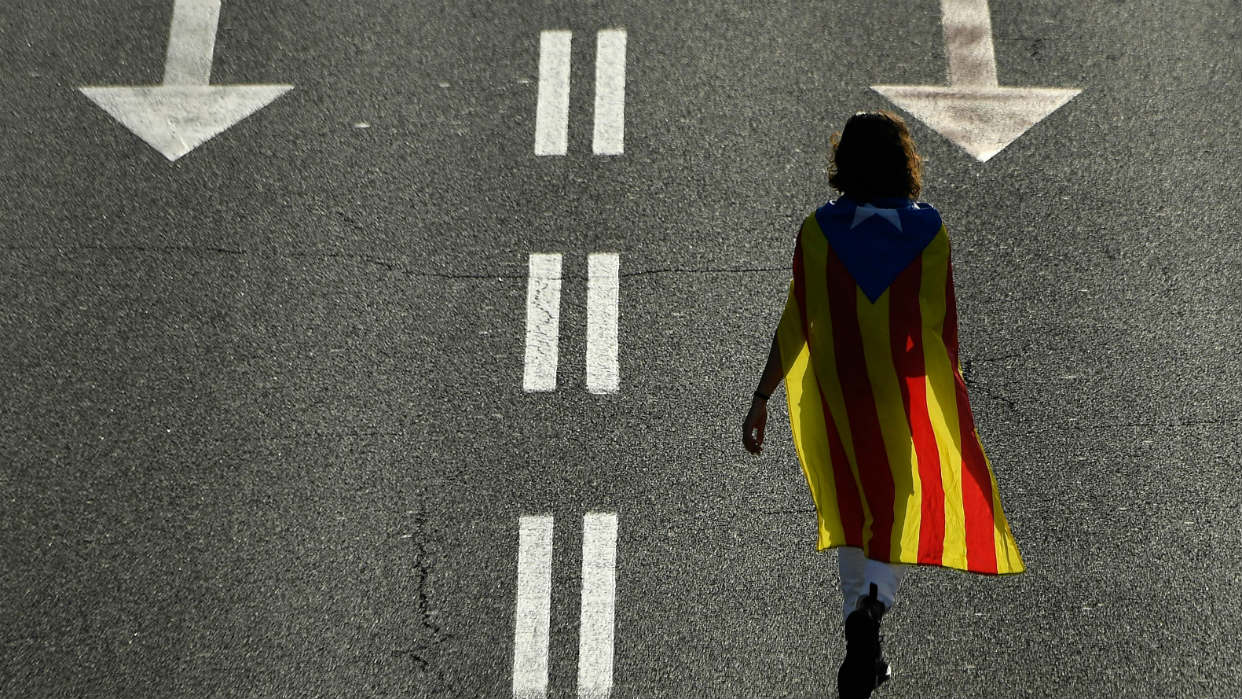
\includegraphics[width=300px]{EU_34981.jpg}%
\newline%
%
Barcelona, España.{-}Una mayoría de diputados del Parlamento regional catalán, principalmente independentistas, aprobó este jueves la apertura de una comisión de investigación sobre la monarquía española, convertida desde hace unos meses en objetivo prioritario de las protestas separatistas.%
\newline%
%
La propuesta de resolución, aprobada con 71 votos a favor y 56 en contra, acuerda investigar "las actividades irregulares o delictivas de personas vinculadas a la Familia Real" aunque, según la oposición, esto sobrepasa las competencias de la cámara regional, destaca AFP.%
\newline%
%
En concreto, la comisión quiere estudiar si el rey Felipe VI presionó a empresas catalanas para que trasladaran su sede social a otras partes de España durante el intento de secesión de 2017 como denunció un diario nacionalista meses atrás y las sospechas de que el rey emérito Juan Carlos I ocultó en el extranjero parte de su patrimonio, así como las supuestas "estructuras de corrupción" vinculadas a la Casa Real.%
\newline%
%
La oposición sostuvo que las comisiones de investigación del Parlamento regional deben circunscribirse a aquellos ámbitos de su competencia, entre los que no se encuentra la monarquía.%
\newline%
%
Históricamente poco popular en esta región, la Casa Real se ha convertido en objetivo de las protestas de los independentistas, que suelen recibir las visitas del rey Felipe VI a Cataluña con manifestaciones, en ocasiones accidentadas.%
\newline%
%
Principalmente le reprochan su discurso del 3 de octubre de 2017, dos días después del referendo ilegal de autodeterminación, cuando acusó de "deslealtad" al independentismo y pidió a los poderes estatales "asegurar el orden constitucional", sin hacer mención a los heridos durante la votación por las cargas policiales.%
\newline%
%
\end{document}